\documentclass[a4j]{jarticle}

\usepackage[dvipdfmx]{graphicx}
\usepackage{url}
\usepackage{here}
\usepackage{listings}
\usepackage{amsmath,amssymb}
\usepackage[dvipdfmx]{color}

\setlength{\headsep}{-5mm}
\setlength{\oddsidemargin}{0mm}
\setlength{\textwidth}{165mm}
\setlength{\textheight}{230mm}
\setlength{\footskip}{20mm}

\title{
\vspace{30mm}
{\bf 子育て支援システム}
\\
\vspace{5mm}
{\bf システム提案書v1\\
}
\vspace{120mm}
}

\author{
\vspace{5mm}
チーム名 007\\
\vspace{5mm}
}


\begin{document}
\maketitle
\tableofcontents
\newpage

\section{はじめに}
近年、女性の社会進出などの労働環境の変化に伴い、夫婦の共働きが増加しています。それにより、保育園の待機児童が増加し親の育児負担が大きくなっています。また、こういった社会の変化に伴い、親同士のコミュニケーションが減少しています。このような親の負担の軽減、親同士のコミュニケーション、子どもの発育を目的とした子育て支援システムをご提案します。

\section{現状の課題}
近年、家庭における夫婦の共働き(図\ref{fig:1})\cite{bib:tomo}や核家族化の増加に伴って、保育園や幼稚園などの保育所に預けなければならない児童が増えています。しかし、保育所の利用率が図\ref{fig:2}に示すように1・2歳児だけでも平成22年から平成29年にかけて29.5\%から45.7\%と約1.5倍に増えているのに対して待機児童の数は平成29年現在でも約2万6千人と変わらないことから、保育所に預けられる児童の数に限りがあるにも関わらず保育所が不足していることが分かります\cite{bib:taiki}。また、図\ref{fig:3}に示すように、待機児童のうち7都府県・指定都市・中核市における待機児童が全体の72.1\%を占めていることから、待機児童の増加は都心部を中心に深刻化していることも分かります\cite{bib:taiki}。他にも、夫婦の共働きは近所の親同士のつながりが減少する要因にもなり、親の空き時間や親子の時間などといったプライベートのための時間も失われています。「日本のママ白書2017年度版」\cite{bib:mama}の調査では、仲の良いママ友の人数が「0人」と答える人が2014年調査から2017年調査にかけて39.9\%から56.7\%に増えていることが分かっています。

\begin{figure}[H]
\begin{center}
\resizebox{15cm}{!}{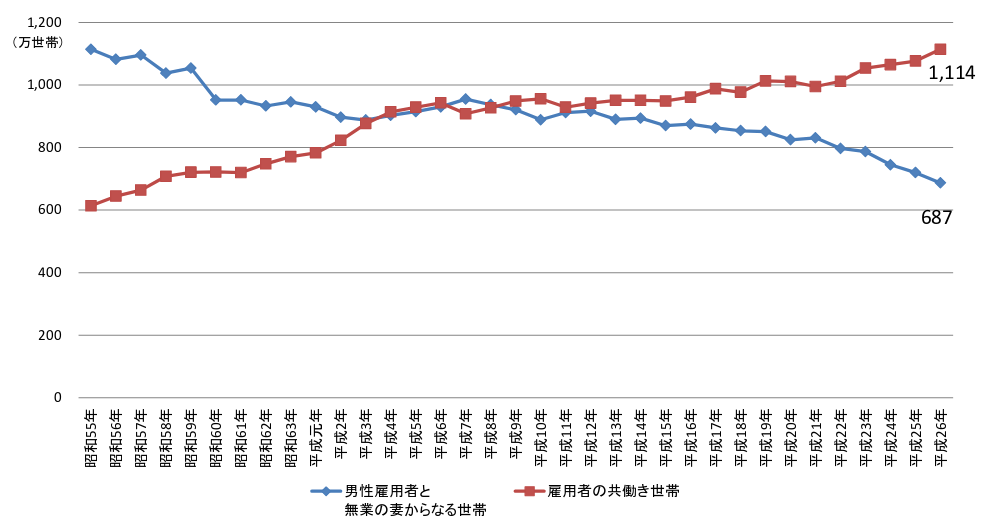
\includegraphics{section2_document1.png}}
\caption{専業主婦世帯と共働き世帯の推移(厚生労働省調べ)}
\label{fig:1}
\end{center}
\end{figure}

\begin{figure}[H]
\begin{center}
\resizebox{15cm}{!}{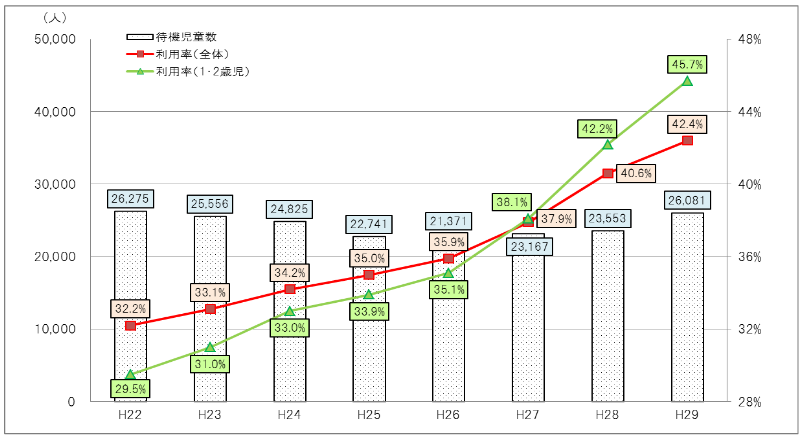
\includegraphics{section2_document2.png}}
\caption{保育所等待機児童数及び保育所等利用率の推移(厚生労働省調べ)}
\label{fig:2}
\end{center}
\end{figure}

\begin{figure}[H]
\begin{center}
\resizebox{15cm}{!}{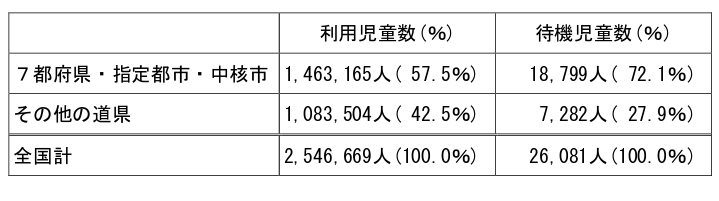
\includegraphics{section2_document3.png}}
\caption{都市部とそれ以外の地域の待機児童数(厚生労働省調べ)}
\label{fig:3}
\end{center}
\end{figure}

これらの現状から以下のような課題があげられます。

\begin{itemize}
\item 親同士のつながりの減少
\item 親子及び親自身のプライベートな時間の不足
\end{itemize}

これらの課題を解決するシステムを提案することで、共働きをする親を中心に親同士のつながりの増加、親の空き時間や親子の時間の確保を目指します。


\section{課題解決のための方法}
この子育て支援システムによる、課題解決方法について説明します。
\begin{itemize}
  \item 利用者のスマートフォンを利用した親同士の交流支援 ~\\
    幼児知育における不安や疑問をシステム利用者間で質問・相談することができる場を提供します。さらに利用者が任意に住んでいる地域を設定することで、その地域に特化した具体的な意見等を共有することができます。
  \item 親子のコミュニケーションを図るための知育ゲーム ~\\
    利用者の端末に幼児向けの知育ゲームを導入することで、親子交流及び知育を行う場を提供します。開発側が幼児向けの知育をサポートすることで、共働きなどで自分の空き時間が少ない親の育児負担を軽減させることにも有効であると考えられます。一方で、親が知育ゲームばかりをさせてしまわないように、これらのコンテンツの利用に対してある程度の時間的制限をかける機能を付けます。また、これらのゲームのうち、塗り絵などの競争性の低いコンテンツに対しては作品(記録)の共有機能をつけます。
\end{itemize}

\section{機能概要・前提条件・制約事項}

\subsection{機能概要}
このシステムは以下の機能を導入します。
\begin{itemize}
\item アカウント機能 ~\\
利用者(親or子)のアカウントをデータベースに登録します。
\item SNS機能 ~\\
親同士が情報交換できるコミュニティ参加型のSNSです。また、個人同士が連絡を取れるプライベートのSNSとコミュニティに質問できる機能もあります。
\item 成長記録機能 ~\\
利用者の写真やゲームの記録等を日付を記載して保存できる機能です。
\item ゲーム機能 ~\\
2~5歳を対象とした簡単な知育ゲームです。
\end{itemize}

\subsection{前提条件}
\begin{itemize}
  \item 個人向け
  \begin{itemize}
    \item インターネットの設備が整っている
    \item Android搭載のスマートフォン・タブレット対応
    \item 日本語対応
  \end{itemize}
\end{itemize}

\subsection{制約事項}

\begin{itemize}
\item 利用者はアカウント情報を正確に登録
\item セキュリティの保証
\item 悪意のある利用者の使用を禁止

\end{itemize}

\section{情報・金銭の流れ}

\subsection{情報の流れ}
子育て支援システムの利用による情報の流れを図\ref{info}に示します。		%子育て支援(システムorシステム)?

システム内で提供されているゲームで遊ぶと結果が記録されます。記録した結果は、親がいつでも確認することができます。親は子育て支援システムを利用している他の親と、子育てに関する情報の共有を行います。システムの機能に不具合があった場合は、利用者が管理人に連絡できるようになっています。管理人は新しいゲームなどの追加コンテンツの提供、システムの修正を行います。システムに広告を提供できる企業は、子育てや幼児教育に関する事業を行っている企業に限定します。これによりシステムの利用者は、子育てに関連する有益な情報を広告からも得ることができます。
%今井は「システム」と略して記述しました。統一すべき。
\begin{figure}[h]
  \begin{center}
    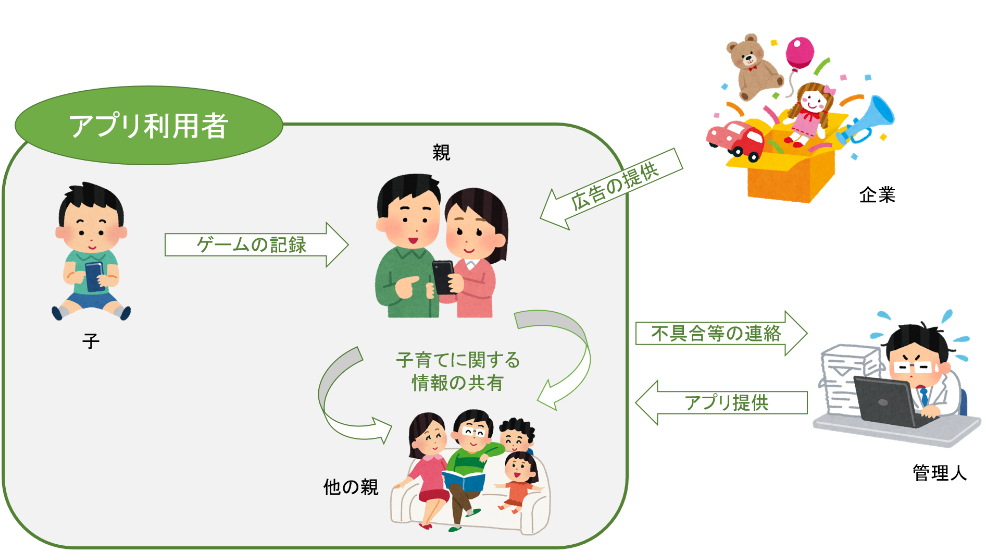
\includegraphics[width = 14cm, height = 9cm]{section5_info.png}
    \caption{情報の流れ}
    \label{info}
  \end{center}
\end{figure}

\newpage
\subsection{金銭の流れ}
子育て支援システムの利用による金銭の流れを図\ref{money}に示します。

子育て支援システムは有料提供を行います。システム内で広告を提供している企業は、管理人に広告費用を支払います。システム利用者がシステム内に表示されている広告商品の購入等を行うことにより、広告を提供している企業側の売上が見込めます。

\begin{figure}[h]
  \begin{center}
    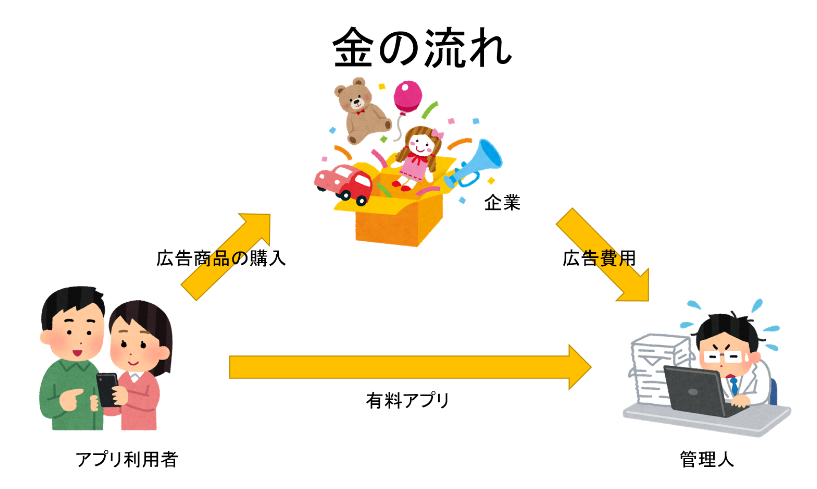
\includegraphics[width = 14cm, height = 9cm]{section5_money.png}
    \caption{金銭の流れ}
    \label{money}
  \end{center}
\end{figure}

\section{利用者}
このシステムが想定する利用者は次の通りです。

\begin{itemize}
\item 2~5歳の幼児\\
  親の家事をする時間などに知育ゲームを利用
\item 2~5歳の幼児の親\\
  SNSを用いた親同士のつながりに利用
\end{itemize}

\section{ハードウェア・ソフトウェア構成}
システムは、サービスのメイン処理を行う管理サーバを1台使用し、クライアントが利用するスマートフォンやタブレット端末と通信を行うことによって、データの送受信や記録を行えるようにします。これを実現するためには、表\ref{tbl: table_hardware}のような構成のハードウェアが必要となります。また、このサービスを提供するためには、表\ref{tbl: table_software}のようなソフトウェア構成が必要となります。

\begin{table}[H]
    \caption{ハードウェア構成}
    \label{tbl: table_hardware}
    \begin{center}
        \begin{tabular}{|c|c|c|} \hline
            項目 & 種類 &  個数\\ \hline
            メインサーバPC & 8TBのレンタルサーバ & 1\\ \hline
            クライアント側端末 & 各個人のスマートフォン・タブレット  & - \\ \hline
        \end{tabular}
    \end{center}
\end{table}


\begin{table}[H]
    \caption{ソフトウェア構成}
    \label{tbl: table_software}
    \begin{center}
        \begin{tabular}{|c|} \hline
            項目 \\ \hline
            Androidスマートフォン・タブレット向けアプリケーション \\ \hline
            管理者向けウェブページ \\ \hline
            サーバ用データベースシステム \\ \hline
        \end{tabular}
    \end{center}
\end{table}

\section{費用と効果}
アプリの開発及び運用にかかる費用は以下の通りです。
 \begin{table}[htp]
\begin{center}
  \caption{開発に要する費用概算}
  \begin{tabular}{|l|r|l|r|l|}\hline
    項目& 単価(円) & 数量 & 金額(円) & 備考  \\ \hline
    Android端末(本体)& 30,000 & 3台 & 90,000 &   \\ \hline
    Android端末(通信料)& 100,000 & 1台分 & 100,000 & 1台のみインターネット通信を試行するため  \\ \hline
    システム開発人件費& 40,000 & 420人日 & 16,800,000 & 工程内訳:7人×2ヶ月(60日)  \\ \hline
    サーバー代& 250,000 & 1台 & 250,000 &   \\ \hline
    維持費& 1,000,000 & 5年 & 5,000,000 &     \\ \hline
    \multicolumn{3}{|l|}{合計} & 22,240,000 &  \\ \hline
  \end{tabular}
\end{center}
\end{table}

このアプリを運用することにより待機児童の知育不足や親同士でのつながりの減少を解決することできると想定されます。このアプリは300円の有料アプリでGooglePlayで配信した場合、手数料として全体の3割が引かれます。全国の2~5歳児の子どもを持つ親を対象としており、その内の3\%となる約12万人の方がダウンロードすると仮定した算出結果は以下のようになります。

\begin{equation}
  120,000×300×0.7 = 25,200,000 [円/年]
\end{equation}

開発と運用にかかる費用と照らし合わせると2,960,000円の黒字となり利益を出すことができます。\par
また、この結果は1年間運用した場合の結果であり、出生率を見ると毎年約90万人近くの子どもが産まれているため5年間運用した場合

\begin{equation}
  228,000×300×0.7 = 47,880,000 [円/5年]
\end{equation}

となるためさらなる利益が期待できると考えられます。



\section{開発体制と工程計画}
このシステムは、7名のプログラマによって実施します。\par
また、システムの工程計画は以下の通りとなっています。

\begin{table}[!h]
  \centering
  \caption{システムの工程計画}
  \begin{tabular}{|c|c|}
    \hline
    \multicolumn{1}{|c|}{工程} & \multicolumn{1}{c|}{完了予定日程} \\ \hline \hline
    仕様凍結 & 2018年10月25日  \\ \hline
    外部設計完了 & 2018年11月22日  \\ \hline
    内部設計完了 & 2018年12月13日 \\ \hline
    開発・動作試験 & 2019年1月17日  \\ \hline
    納品 & 2019年1月24日  \\ \hline
  \end{tabular}
\end{table}


\section{このシステム提案のアピールポイント}
\begin{description}
\item[(1)] 親の家事などの合間に子どもたちに利用してもらうため親の負担を軽減できることが考えられます。
\item[(2)] 知育ゲームによって子どもの考える力を伸ばすことができます。
  
\item[(3)] 子どもの発育を促すだけでなく、子どものゲームの記録を残すことができるため親が子どもの日々の成長過程をいつでも見ることが可能となります。
\item[(4)] SNS機能を設けているため、親同士のコミュニケーションがとりやすくなることが考えられます。さらに質問箱などの機能も設けているため、子どもが熱を出したときの対処等を聞くなど親同士でのサポートが可能となります。
\end{description}



\begin{thebibliography}{3}
\bibitem{bib:tomo}
  専業主婦世帯と共働き世帯の推移.\\
  \url{https://www.mhlw.go.jp/file/05-Shingikai-11201000-Roudoukijunkyoku-Soumuka/0000118655.pdf}.
  \newblock 2018年10月11日閲覧.

\bibitem{bib:taiki}
  保育所等関連状況取りまとめ(平成29年4月1日).\\
  \url{https://www.mhlw.go.jp/file/04-Houdouhappyou-11907000-Koyoukintoujidoukateikyoku-Hoikuka/0000176121.pdf}.
  \newblock 2018年10月11日閲覧.

\bibitem{bib:mama}
  日本のママ白書2017年度版.\\
  \url{https://www.mindshare.co.jp/mama/whitepaper2017/}.
  \newblock 2018年10月11日閲覧.
\end{thebibliography}

\end{document}
